\subsubsection{Guidance method's questionnaire.}
\label{subsec:results_questionnaires}

Finally, the Questionnaire is analyzed to give an idea about the impressions of the users with each device. This is an important evaluation to seek their impressions of each method. The higher the score, the more the user was satisfaction with that method. The Table \ref{tab:questionnaire_average_blind} shows the score of each method and they are plotted in the Figure \ref{fig:barplot_questionnaire_scene_blind}. The Figure show a disatisfaction with the haptic devices alone.


\begin{table}[!htb]
\centering
\caption{ Guidance method questionnaire score felled by the blinded participants.}
\label{tab:questionnaire_average_blind}
\begin{tabular}{llrrrrr}
\toprule
{} &  Audio &  \begin{tabular}[c]{@{}l@{}}Haptic\\ Belt\end{tabular} &  \begin{tabular}[c]{@{}l@{}}Virtual\\ Cane\end{tabular} &  Mixture \\
Participant &        &                                                        &                                                         &          \\
\midrule
001C        &  0.774 &                                                  0.543 &                                                   0.629 &    0.865 \\
002C        &  0.857 &                                                  0.743 &                                                   0.543 &    0.935 \\
003C        &  0.929 &                                                  0.571 &                                                   0.543 &    0.745 \\
004C        &  0.881 &                                                  0.486 &                                                   0.400 &    0.730 \\
\bottomrule
\end{tabular}
\end{table}



\begin{figure}[!htb]
    \centering
    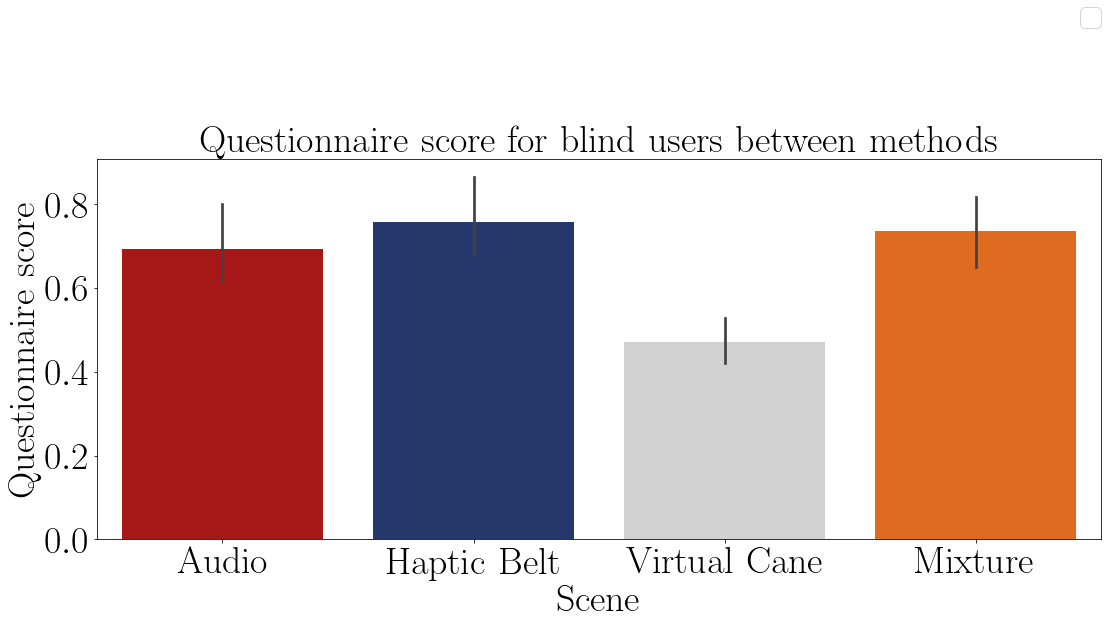
\includegraphics[width = 0.8\linewidth]{Resultados/Questionario/Figuras/png/barplot_questionnaire_scene_blind.png}
    \caption{Barplot of the average questionaire score of the blind participants on each method.}
    \label{fig:barplot_questionnaire_scene_blind}
\end{figure}

\begin{figure}[!htb]
    \centering
    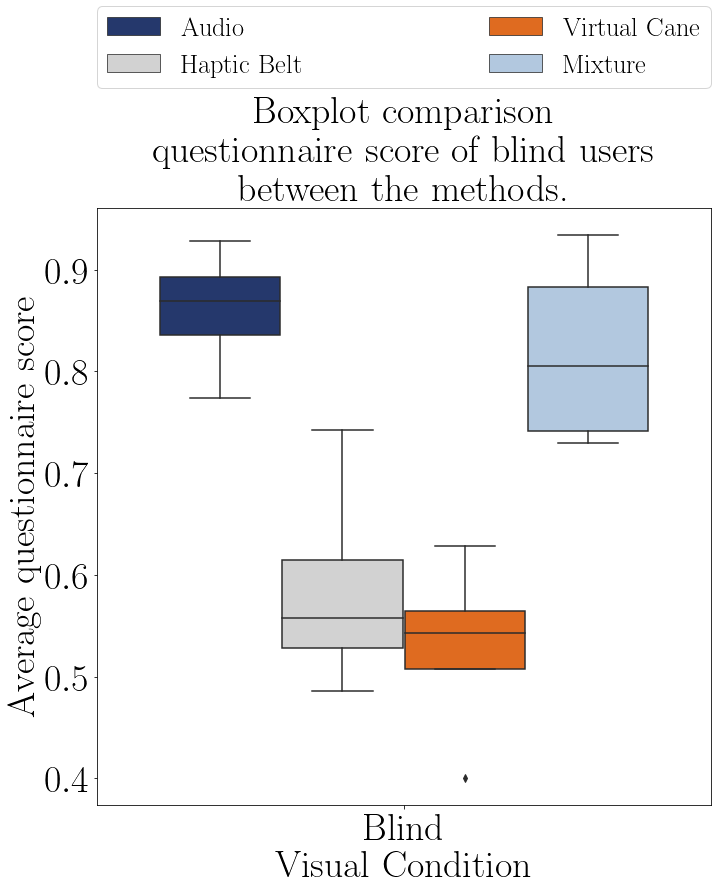
\includegraphics[width = 0.6\linewidth]{Resultados/Questionario/Figuras/png/boxplot_questionnaire_scene_blind.png}
    \caption{Boxplot of the questionaire score of the blind participants grouped by method.}
    \label{fig:boxplot_quest_blind_scene}
\end{figure}

The Table \ref{tab:questionnaire_average_group_blind} show the the average questionnaire score on each method. It also shows a disatisfaction with the haptic devices alone.


\begin{table}[!htb]
\centering
\caption{Guidance method questionnaire average score for the blind participants.}
\label{tab:questionnaire_average_group_blind}
\begin{tabular}{lrrrrr}
\toprule
{} & Audio & Haptic Belt & Virtual Cane & Mixture \\
Visual Condition &       &             &              &         \\
\midrule
Blind            &  0.86 &        0.59 &         0.53 &    0.82 \\
\bottomrule
\end{tabular}
\end{table}



The Figures \ref{fig:qqplot_sagat_avg_two_way} and \ref{fig:residplot_sagat_avg_two_way} shows the distribution and variance of the Table \ref{tab:sagat_table_blind}. These Figures shows that the data are normally distributed and that the methods have a similar variance.
The Table \ref{tab:blocanova_sagat_avg_two_way} shows the Anova test p-value of the SAGAT score of the "blind" sample. The p-values indicates that the method have influence on the questionnaire score. Meaning that the participants had differents level os satisfaction about each method.


\begin{table}[!htb]
\centering
\caption{Anova p-value for the questionnaire score on each method for blinded users.}
\label{tab:blocanova_questionnaire}
\begin{tabular}{lrrrrr}
\toprule
               Source &  Squared sum &  DOF & Squared average &      F & \begin{tabular}[c]{@{}l@{}}P-Value \\ $(F_{0} > F)$\end{tabular} \\
\midrule
Participants (blocks) &        0.042 &    3 &           0.110 &  2.014 &                                                                  \\
               Method &        0.329 &    3 &           0.014 & 15.677 &                                                          0.001** \\
   Experimental error &        0.063 &    9 &           0.007 &        &                                                                  \\
                Total &        0.434 &   15 &                 &        &                                                                  \\
\bottomrule
\end{tabular}
\end{table}



\begin{figure}[!htb]
    \centering
    \begin{minipage}{0.45\textwidth}
        \centering
        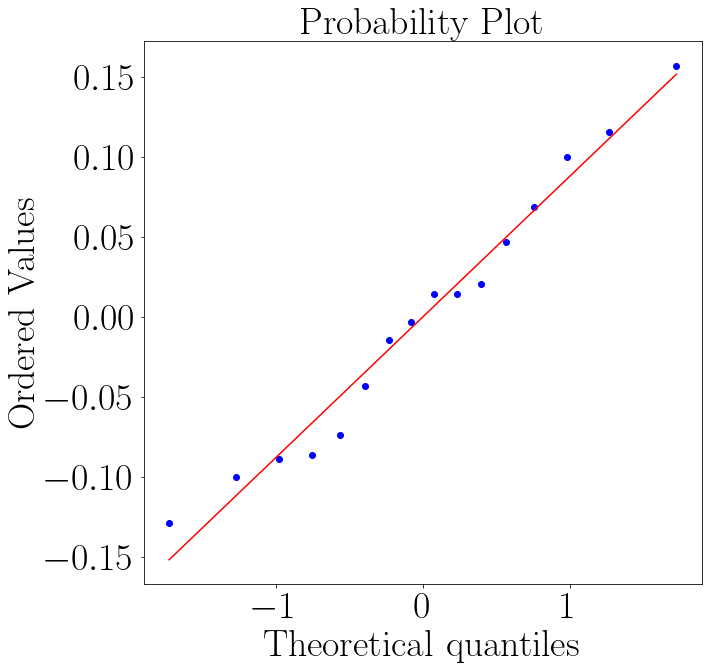
\includegraphics[width = 0.8\linewidth]{Resultados/Questionario/Figuras/png/qqplot_questionnaires.png}
        \caption{QQ plot of the questionnaire score of the blind participants on each method.}
        \label{fig:qqplot_sagat_avg_two_way}
    \end{minipage}
    \begin{minipage}{0.45\textwidth}
        \centering
        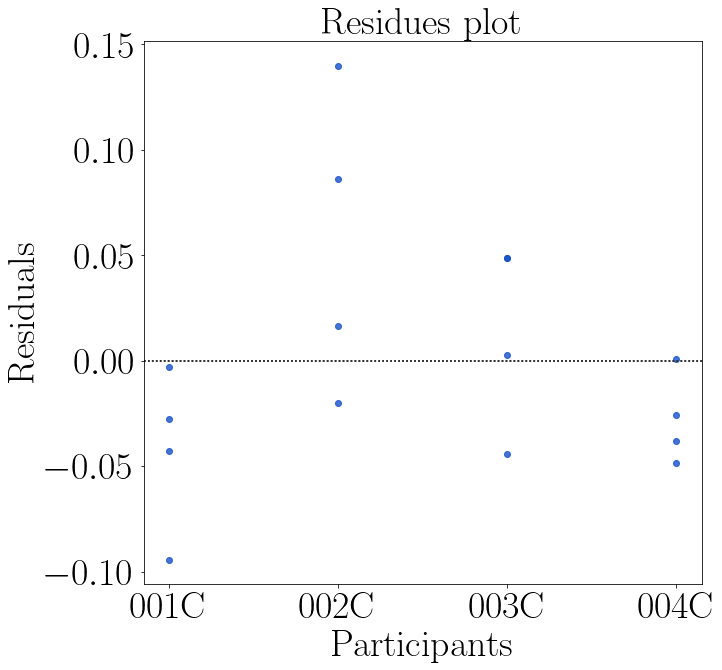
\includegraphics[width = 0.8\linewidth]{Resultados/Questionario/Figuras/png/residplot_questionnaires.png}
        \caption{Residual plot of the questionnaire score the blind participants on each method.}
        \label{fig:residplot_questionnaires}
    \end{minipage}
\end{figure}


The Table \ref{tab:lsd_questionnaire} presents the conclusion of a pairwise Fisher LSD test of the blind NASA-TLX score between all the guidance methods. The results show that only the "Audio" and "Mixture" have the same statistically result and that there is a difference between the both "Haptic Belt" and "Virtual Cane".


\begin{table}[!htb]
\centering
\caption{Cross validation p-value for the questionnaire score on each method for blinded users.}
\label{tab:lsd_questionnaire}
\begin{tabular}{rclr}
\toprule
      \multicolumn{3}{c}{Method} &                                           Analysis \\
\midrule
       Audio & $X$ & Haptic Belt &        $H_1 : \mu_{Audio} \ne \mu_{Haptic Belt}**$ \\
      Audio & $X$ & Virtual Cane &       $H_1 : \mu_{Audio} \ne \mu_{Virtual Cane}**$ \\
           Audio & $X$ & Mixture &                $H_0 : \mu_{Audio} = \mu_{Mixture}$ \\
Haptic Belt & $X$ & Virtual Cane & $H_1 : \mu_{Haptic Belt} \ne \mu_{Virtual Cane}**$ \\
     Haptic Belt & $X$ & Mixture &          $H_0 : \mu_{Haptic Belt} = \mu_{Mixture}$ \\
    Virtual Cane & $X$ & Mixture &     $H_1 : \mu_{Virtual Cane} \ne \mu_{Mixture}**$ \\
\bottomrule
\end{tabular}
\end{table}



The LSD Table \ref{tab:lsd_questionnaire} confirms the information of the Figure \ref{fig:boxplot_quest_blind_scene} that the “Audio” and the ”Mixture” methods were the most favorite by the blind participants, whilst the “Haptic Belt” and “Virtual Cane” were the most unfavorite devices. The participants did comment about those two last devices, saying that they were not precise enough, confusing and very different from what they are used to use.

\FloatBarrier